% !TEX encoding = UTF-8 Unicode

\linespread{1.7}
\chapter{Calibration of the Near-surface Seismic Structure in the SCEC Community Velocity Model Version 4}
\linespread{2.0}
%\newrefsection
\label{chap:vs30}

\graphicspath{{/Users/zhh076/work/PhD_way/vs30/}}

The near-surface seismic structure (to a depth of about 1000 m), particularly the shear-wave velocity (Vs), can strongly affect the propagation of seismic waves, and therefore must be accurately calibrated for ground motion simulations and seismic hazard assessment. The Vs of the top ~30 m of the crust (Vs30) is often well-characterized from borehole studies, geotechnical measurements, and water wells, while the velocities of the material deeper than about 1000 m are typically determined by tomography studies. However, the material parameters between these two regions are typically poorly constrained due to lack of data constraints. A widely-used method for incorporating the near-surface earth structure is incorporated in the Southern California Earthquake Center (SCEC) Community Velocity Models (CVMs) by interpolating Vs from Vs30 measurements to the S-wave velocity at 350 m \citep{elyVs30derivedNearsurfaceSeismic2010}. However, our 3D simulations of the 2014 M5.1 La Habra earthquake in the Los Angeles area using the SCEC CVM-S4.26.M01 model significantly underpredict low-frequency (< 1 Hz) ground motions at rock sites for the \citet{elyVs30derivedNearsurfaceSeismic2010} method. On the other hand, extending the Vs30-based refinement of the shallow velocities down to a depth of about 1000 meters improves the fit between our synthetics and seismic data at rock sites considerably, without compromising the fit at soil sites. We recommend that our proposed near-surface velocity refinement at rock sites down to about 1000 meters be incorporated in CVM-S4.26M01, as well as considered for other CVMs.


%%%%%%%%%%%%%%%%%%%%%%%%%%
\section{Introduction} \label{vs30:intro}
Ground motion amplification due to the near-surface structure is widely accepted and well-studied \citep{gilbertSanFranciscoEarthquake1907,fieldModifiedGroundMotionAttenuation2000}, and needs to be incorporated in numerical  simulations of earthquakes to produce accurate ground motion results. The time-averaged shear-wave velocity (Vs) in the upper 30 m (Vs30) is routinely used as a representation of the site condition in ground motion prediction models and building codes \citep{borcherdtEstimatesSiteDependentResponse1994,bozorgniaNGAWest2ResearchProject2014,internationalcodecouncil2015IBCInternational2014}. For this purpose, several methods have proposed useful methods to derive Vs30 from topography (Wald et al. 2007), supplemented with near-surface geological information (Thompson et al. 2014; Wills et al. 2015). However, with the continuing advancement in the Vs30-based methodologies by the seismic hazard community (e.g., Thompson et al. 2014, Heath et al. 2020), it is clear  that Vs30 is not a good single proxy for the estimation of site amplification (e.g., Steidl 2000, Lee and Trifunac 2010 and Shingaki et al. 2018). One reason is the prohibitive cost of measuring velocity profiles at the resolution needed for seismic hazard analysis, leading to highly approximate results from interpolating limited Vs30 values and combining geological units. Furthermore, Vs30 value is found to be a product complicated by age and grain size, and therefore includes inherent inaccuracy within the soil category classification. Finally, Vs30 cannot account for depth-dependent or lateral velocity variations,  which all affect the seismic wavefields.

While the current approximations to correct for site effects serve an important purpose, a fully physics-based approach for seismic hazard analysis presents itself as a more difficult, but robust, long-term goal. In such an approach, the full wavefield is computed deterministically to maximum frequencies of 5 Hz or higher using a realistic 3D velocity model (e.g., Withers et al. 2019a,b; Hu and Olsen 2021). A necessary ingredient in producing accurate synthetic seismograms using physics-based simulations is an accurate velocity model for the model region. Community Velocity Models (CVMs) have been developed for such purpose, e.g., the Southern California Earthquake Center (SCEC) CVMs (Small et al., 2017), the Cascadia CVM (Stephenson et al., 2017) and the Subsurface Structure Model maintained by the Japan Seismic Hazard Information Station (Fujiwara et al. 2017). These velocity models are often generated by combining 3D tomographic inversion from seismic waves (e.g., Tape et al. 2009,  Lee et al. 2014) with shallow geotechnical information (e.g., Vs30) and often yield a fixed resolution of a few hundreds of meters along depth. The spatial resolution of large-scale tomographic studies is generally limited by the density of ray paths, particularly in the upper ~1000 m of the crust. While a relatively coarse resolution may be acceptable for the lower crust, that is insufficient to resolve shallower, more complicated structures with more rapid velocity variation. Unfortunately, data constraints on the velocities for the material between depths of about 30 m and 1000 m are limited to relatively rare seismic refraction studies (e.g. Teague et al. 2018) or borehole logs (e.g, Stellar 1996, Thompson  2012).

Previous studies have attempted to bridge the data constraints at shallow (<~30 m) and deeper (>~1000 m) depths for rock sites. For example, Boore and Joyner (1997) generated a continuous depth-dependent Vs function based on 3 different intervals. The Vs profile in the upper 30 m was constructed from interpolated shallow average arrival times. At depths below 4 km, Vs was estimated from the P-wave velocity (Vp), measured from earthquake location studies and velocity surveys, on the assumption of a fixed Poisson ratio at 0.25. Finally, the shallow and deeper Vs were connected using two power-law functions.  Ely et al. (2010) proposed a generalized method that modifies the surface Vs from Vs30 and then interpolates velocities down to 350 m depth, which has been implemented in some of the SCEC CVMs. The Vs30 values adopted by Ely et al. (2010) were obtained from the geology-based Vs30 map of Wills and Clahan (2006) for California and the topography-based estimations by Wald and Allen (2007) outside California. The determination of  350 m used for the depth extent of the Vs refinements by Ely et al. (2010) was based on qualitative comparison between seismic synthetics and data records from the 2008 M5.4 Chino Hills, CA, earthquake.

In this study, we aim to quantify the accuracy of the top 1000 m of crust in the greater Los Angeles area in California using using 3D wavefield simulations of the 2014 M5.1 La Habra earthquake, as well as propose an improved refinement method for rock site, if needed. The paper is organized as follows: we first briefly introduce our numerical approach to obtain the simulated ground motions, present an approximate 1D analysis of site amplification to evaluate the potential to improve site amplification at rock sites, and finally evaluate different rock site refinements using 3D wave propagation simulation and provide our recommendation.



%%%%%%%%%%%%%%%%%%%%%%%%%%%%%%%
\section{Numerical Approach}\label{vs30:approach}


%%%%%%%%%%%%%%%%%%%%%%%%%%%%%%


\section*{Data and Resources}
The UCVM program used to extract velocity meshes can be obtained from SCEC on \url{https://github.com/SCECcode/UCVMC} (last accessed 12/2020). The simulations were performed on Summit at the Oak Ridge Leadership Computing Facility in Tennessee. Most of the data-processing work was done using Python and the Generic Mapping Tools package (\url{https://www.generic-mapping-tools.org}, last accessed 04/2021).


\section*{Acknowledgements}
\addcontentsline{toc}{section}{\protect\numberline{}Acknowledgements}

This research was supported through the U.S. Geological Survey External Program (award \#G19AS00021), as well as the Southern California Earthquake Center (SCEC; Contribution Number xx). SCEC is funded by the National Science Foundation (NSF) Cooperative Agreement EAR-1600087 and the U.S. Geological Survey (USGS) Cooperative Agreement \url{G17AC00047}. We thank Robert W. Graves for providing the source models and Fabio Silva for providing the station records of the 2014 La Habra earthquake.

\Cref{chap:vs30}, in full, is a reformatted version of a paper under revision for publication: Hu, Z., K. B. Olsen, and S. M. Day (2021). ``Calibration of the Near-surface Seismic Structure in the SCEC Community Velocity Model Version 4.''
The dissertation author was the primary investigator and author of this paper.

\newpage
\section*{Tables and Figures}
\addcontentsline{toc}{section}{\protect\numberline{}Tables and Figures}%

%% For very long table
% \clearpage
% \begin{sidewaystable}[!ht]
% \caption{Coregionalization matrix $\mathbf{P}^\mathbf{3}$}
% \begin{adjustbox}{width=\textwidth,center}
% \begin{tabular}{|c|cccccccccccccccccccccccccccccccc|c|}
% \end{tabular}
% \label{tb:5-S3}
% \end{adjustbox}
% \end{sidewaystable}


\clearpage
\begin{table}[!ht]
  \vrule depth12pt width 0pt
  \caption{Simulation parameters used for the deterministic ground motion simulations of the 2014 La Habra earthquake.}
  \label{tab:vs30-1}
  \begin{tabular}{@{}lc@{}}
    \toprule
    \textbf{Domain}               & \multicolumn{1}{l}{}      \\ \midrule
    Length                        & 147.840 km                \\
    Width                         & 140.400 km                \\
    Depth                         & 58.000 km                 \\
    Southwest corner              & \begin{tabular}[c]{@{}c@{}}-118.9774168,\\ 33.9093124\end{tabular} \\ \midrule
    \textbf{Spatial resolution}   &                           \\ \midrule
    Maximum frequency             & 5 Hz                      \\
    Minimum $V_S$                 & 500 m/s                   \\
    Points per minimum wavelength & 5                         \\
    Grid discretization           & 20/60 m                   \\
    Number of cells               & 25,092,587,520            \\
    Number of GPU processors      & 960                       \\
    Wall-clock time               & 1.5 hr                    \\ \midrule
    \textbf{Temporal resolution}  &                           \\ \midrule
    Time discretization           & 0.001 s                   \\
    Simulation time               & 120 s                     \\
    Number of timesteps           & 120,000                   \\ \bottomrule
  \end{tabular}
\end{table}


\clearpage
\begin{table}[!ht]
  \vrule depth12pt width 0pt
  \caption{Rock site information}
  \label{tb:vs30-2}
  \resizebox{0.85\columnwidth}{!}{%
    \begin{tabular}{@{}ccccccc@{}}
      \toprule
      site\_name & Lon (\textdegree) & Lat (\textdegree) & $R_{hypo}$ (km) & $V_S$ (m/s) & $V_{S30}$ (m/s) & Elevation (m) \\ \midrule
      CISRN      & -117.79           & 33.83             & 17.53           & 1908.44     & 351.90          & 212.32        \\
      CIQ0029    & -117.75           & 33.73             & 27.87           & 2163.35     & 293.50          & 94.84         \\
      CE13220    & -117.75           & 33.68             & 31.99           & 2090.55     & 351.90          & 70.28         \\
      CISTG      & -117.77           & 33.66             & 32.61           & 1980.29     & 351.90          & 47.53         \\
      CE13441    & -117.78           & 33.66             & 32.74           & 1934.54     & 447.28          & 45.87         \\
      CIPLS      & -117.61           & 33.80             & 33.36           & 2234.93     & 351.90          & 1215.81       \\
      CE24399    & -118.06           & 34.22             & 36.28           & 2597.01     & 710.10          & 1724.74       \\
      CIMWC      & -118.06           & 34.22             & 36.28           & 2596.96     & 710.10          & 1727.73       \\
      CIQ0034    & -117.66           & 33.69             & 36.56           & 2289.27     & 293.50          & 324.50        \\
      CIQ0009    & -117.71           & 33.61             & 41.12           & 1885.40     & 351.90          & 106.23        \\
      CIQ0022    & -117.50           & 33.77             & 43.52           & 2425.56     & 351.90          & 362.41        \\
      CIBFS      & -117.66           & 34.24             & 44.01           & 2270.57     & 710.10          & 1301.77       \\
      NP707      & -117.45           & 33.85             & 45.57           & 2913.91     & 293.50          & 407.88        \\
      CIQ0026    & -117.57           & 33.64             & 45.83           & 2529.13     & 228.20          & 375.70        \\
      CIQ0005    & -117.77           & 33.53             & 46.38           & 1961.18     & 710.10          & 42.60         \\
      CISDD      & -117.66           & 33.55             & 48.13           & 1923.53     & 351.90          & 122.19        \\
      CIQ0038    & -117.43           & 33.73             & 51.38           & 2926.22     & 293.50          & 416.98        \\
      CE13916    & -117.32           & 33.90             & 56.71           & 2893.67     & 518.90          & 522.59        \\
      CITA2      & -117.68           & 34.38             & 56.88           & 2381.10     & 351.90          & 2258.42       \\
      CILPC      & -117.55           & 34.32             & 56.89           & 1970.65     & 351.90          & 1344.56       \\
      CICJM      & -117.42           & 34.27             & 61.30           & 2404.97     & 228.20          & 1615.85       \\
      CE13080    & -117.25           & 33.97             & 63.28           & 2607.63     & 518.90          & 542.10        \\
      CE23958    & -117.65           & 34.44             & 63.85           & 2093.92     & 447.28          & 1236.29       \\
      CIQ0035    & -118.20           & 34.47             & 66.03           & 2428.36     & 710.10          & 864.55        \\
      CE13096    & -117.27           & 33.70             & 66.46           & 4105.94     & 518.90          & 426.84        \\
      CE23292    & -117.54           & 34.43             & 66.98           & 1807.64     & 710.10          & 1211.92       \\
      CIIPT      & -117.29           & 34.20             & 67.45           & 2552.72     & 228.20          & 945.86        \\
      CIPER      & -117.21           & 33.86             & 67.67           & 2880.41     & 518.90          & 467.03        \\
      CIQ0028    & -117.18           & 33.83             & 70.30           & 3197.89     & 518.90          & 461.22        \\
      CIQ0013    & -118.06           & 34.54             & 70.31           & 2620.60     & 518.90          & 859.30        \\
      CE13927    & -117.17           & 33.92             & 70.31           & 2377.65     & 351.90          & 494.08        \\
      CISOF      & -117.56           & 33.37             & 70.35           & 2333.99     & 351.90          & 16.09         \\
      CILUG      & -117.37           & 34.37             & 72.20           & 2080.27     & 513.69          & 1136.43       \\
      CISBPX     & -117.24           & 34.23             & 73.34           & 2310.65     & 293.50          & 1872.13       \\
      CE13924    & -117.13           & 33.75             & 76.98           & 4161.26     & 351.90          & 486.31        \\
      CIQ0049    & -117.13           & 34.20             & 80.69           & 2184.64     & 710.10          & 1661.03       \\
      CIBBS      & -116.98           & 33.92             & 88.03           & 1639.46     & 518.90          & 782.79        \\
      CE12919    & -116.97           & 33.93             & 88.77           & 1559.19     & 518.90          & 795.50        \\
      CIQ0020    & -116.95           & 33.96             & 90.66           & 1588.16     & 468.40          & 859.36        \\
      \bottomrule
    \end{tabular}}
\end{table}


\clearpage
\begin{table}[!ht]
  \begin{threeparttable}
    \vrule depth12pt width 0pt
    \centering
    \caption{Average FAS biases for all three components for various models.}
    \label{tab:vs30-3}
    \resizebox{\textwidth}{!}{%
      \renewcommand{\arraystretch}{1.4}%
      \begin{tabular}{@{}ccccccccc@{}}
        \toprule
        \multirow{2}{*}{Model}                    & \multicolumn{4}{c}{Soil sites} & \multicolumn{4}{c}{Rock sites}                                                                       \\ \cmidrule(l){2-9}
                                                  &
        East-west                                 &
        North-south                               &
        Vertical                                  &
        \textbf{Average}                          &
        East-west                                 &
        North-south                               &
        Vertical                                  &
        \textbf{Average}                                                                                                                                                                  \\ \cmidrule(r){1-1} \cmidrule(l){2-9}
        CVM-S\tnote{\textsuperscript{*}}          & 0.034                          & 0.044                          & 0.009 & \textbf{0.029} & -0.277 & -0.261 & -0.136 & \textbf{-0.225} \\
        CVM-S + 350 m\tnote{\textsuperscript{*}}  & 0.040                          & 0.048                          & 0.009 & \textbf{0.033} & -0.171 & -0.153 & -0.138 & \textbf{-0.154} \\
        CVM-S + 700 m\tnote{\textsuperscript{*}}  & 0.055                          & 0.062                          & 0.018 & \textbf{0.045} & -0.020 & -0.015 & -0.087 & \textbf{-0.041} \\
        CVM-S + 1000 m\tnote{\textsuperscript{*}} & 0.065                          & 0.073                          & 0.020 & \textbf{0.053} & 0.048  & 0.055  & -0.055 & \textbf{0.016}  \\
        \begin{tabular}[c]{@{}c@{}}CVM-S + 350 m \\[-5pt] + $Q_S=0.05V_S$\tnote{\textdagger}\end{tabular}                 &
        -0.039                                    &
        -0.027                                    &
        -0.091                                    &
        \textbf{-0.052}                           &
        -0.064                                    &
        -0.052                                    &
        -0.156                                    &
        \textbf{-0.091}                                                                                                                                                                   \\
        \begin{tabular}[c]{@{}c@{}}CVM-S + 1000 m \\[-5pt] + $Q_S=0.15V_S$\tnote{\textdagger}\end{tabular}                 &
        0.085                                     &
        0.091                                     &
        0.061                                     &
        \textbf{0.080}                            &
        -0.135                                    &
        -0.120                                    &
        -0.105                                    &
        \textbf{-0.120}                                                                                                                                                                   \\ \bottomrule
      \end{tabular}
    }
    \begin{tablenotes}
      \item[\textsuperscript{*}] \footnotesize $Q_S=0.1V_S$; $Q_P=2Q_S$\\[-10pt]
      \item[\textdagger] \footnotesize $Q_P=2Q_S$
    \end{tablenotes}
  \end{threeparttable}
\end{table}

% %%%%%%%%%%%%% figures 

\clearpage
\begin{figure}[!ht]
  \centering
  \includegraphics[width=0.9\textwidth]{figures/figure_vs30_1.png}
  \caption{Simulation region for the La Habra event (rectangle) and locations of 259 strong ground motion stations (circles represent soil sites with surface $V_S$ < 1000 m/s and red triangles represent rock sites with surface $V_S$ >= 1000 m/s). The named sites (triangles with black edge) are selected for further comparisons in Figure 12. The star depicts the epicenter of the La Habra earthquake.
  }
  \label{fig:vs30-1}
\end{figure}

\clearpage
\begin{figure}[!ht]
  \centering
  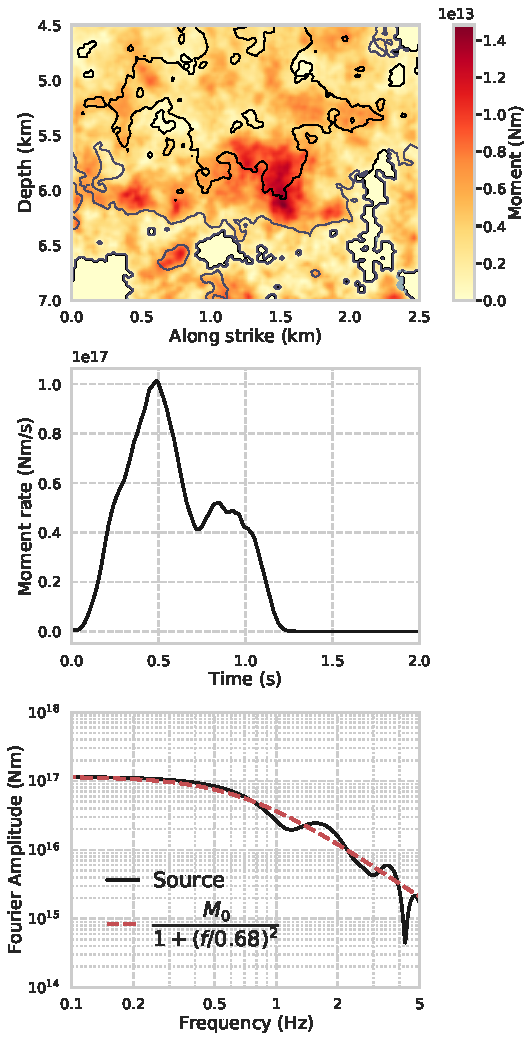
\includegraphics[width=0.9\textwidth,height=0.9\textheight,keepaspectratio]{figures/figure_vs30_2.pdf}
  \caption{Description of the source model used in this study. (a) Total moment on the fault. The contours represent rupture time at a 0.4 s interval starting from 0. (b) and (c) represent the sum of the moment rates for all subfaults and the Fouerier amplitude spectrum, respectively.}
  \label{fig:vs30-2}
\end{figure}

\clearpage
\begin{figure}[!ht]
  \centering
  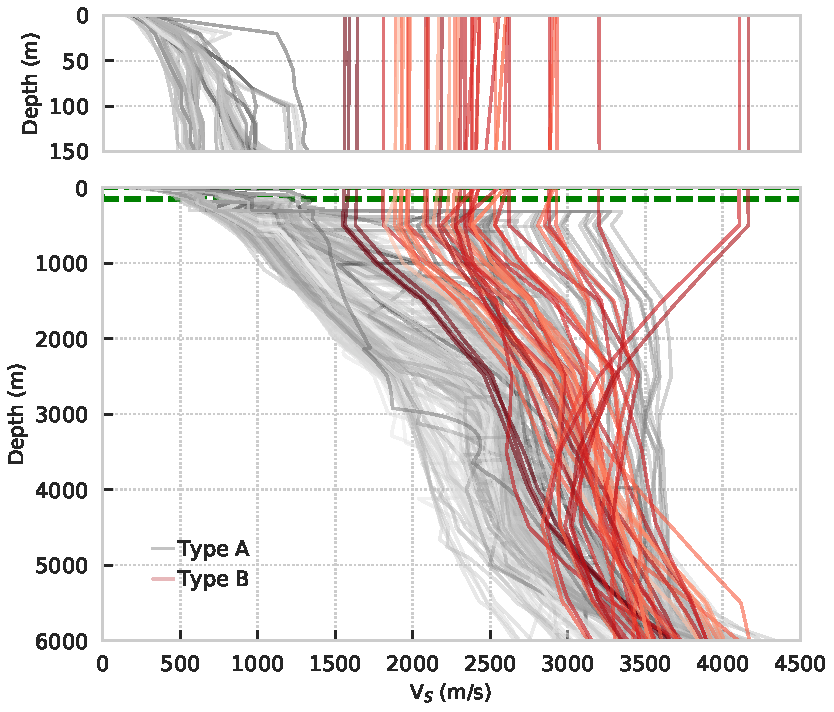
\includegraphics[width=0.9\textwidth]{figures/figure_vs30_3.pdf}
  \caption{(a) Top 150 m and (b) 0-4000 m $V_S$ profiles at the 259 stations. The black and red curves represent rock (surface $V_S$ >= 1000 m/s) and soil (surface $V_S$ < 1000 m/s) sites, respectively. The darker curves denote the sites with farther distance from the source.}
  \label{fig:vs30-3}
\end{figure}

\clearpage
\begin{figure}[!ht]
  \centering
  \includegraphics[width=0.9\textwidth]{figures/figure_vs30_4.pdf}
  \caption{FAS derived from the records (black) and CVM-S (blue) for the (a) east-west component, (b) north-south component and (c) vertical component. The left and right columns represent soil sites with surface $V_S$ smaller and larger than 1000 m/s, respectively. The solid line is the median of FAS over the site group, the narrow band is the 95\% confidence interval of the median, and the wide band depicts the standard deviation centered at the median.
  }
  \label{fig:vs30-4}
\end{figure}

\clearpage
\begin{figure}[!ht]
  \centering
  \includegraphics[width=0.9\textwidth]{figures/figure_vs30_5.png}
  \caption{(a) Surface $V_S$ extracted from CVM-S, and (b) $V_{S30}$ from \citet{thompsonUpdatedVs30Map2018} in our model domain (values in the left bottom corner are not available). The star denotes the epicenter.}
  \label{fig:vs30-5}
\end{figure}

\clearpage
\begin{figure}[!ht]
  \centering
  \includegraphics[width=0.9\textwidth]{figures/figure_vs30_6.pdf}
  \caption{Representative $V_S$ profiles for (a) soil sites and (b) rock sites from CVM-S. The thick black curves depict the averaged velocity profiles for all 220 soil and 39 rock sites directly extracted from CVM-S. The thin lines show the $V_S$ refinement resulting from our proposed method for different $z_T$ depths between 200 m and 1500 m. The dashed curve shows the $V_S$ profile calculated using our preferred $z_T$ value of 1000 m.}
  \label{fig:vs30-6}
\end{figure}

\clearpage
\begin{figure}[!ht]
  \centering
  \includegraphics[width=0.9\textwidth]{figures/figure_vs30_7.pdf}
  \caption{The SH1D response for the refined profiles using various $z_T$ depths for average (a) soil and (b) rock sites, divided by the response obtained with the averaged soil and rock profiles from CVM-S.}
  \label{fig:vs30-7}
\end{figure}

\clearpage
\begin{figure}[!ht]
  \centering
  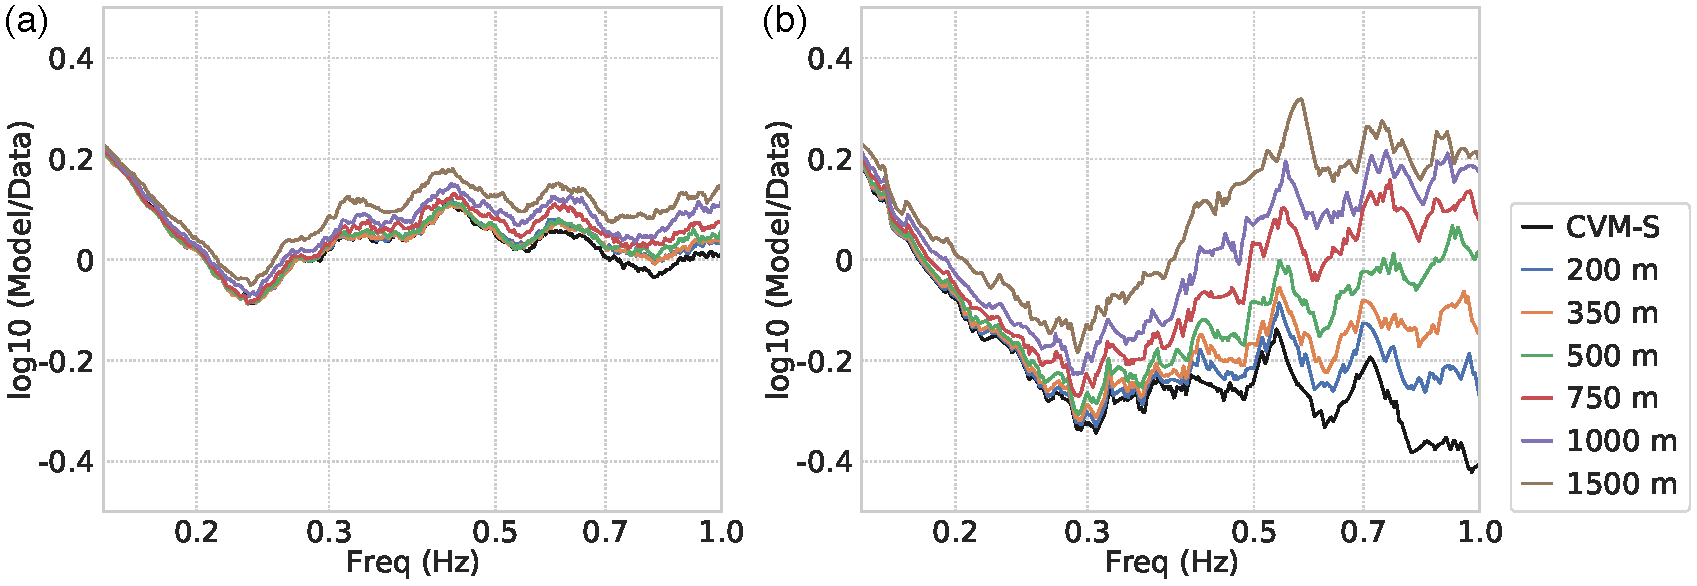
\includegraphics[width=0.9\textwidth]{figures/figure_vs30_8.pdf}
  \caption{Bias of FAS for the two horizontal components averaged over all (a) soil and (b) rock sites for CVM-S at all 259 stations, superimposed with the corresponding SH1D response. The black curves denote CVM-S and other labeled curves represent refinements to various depths using SH1D results.}
  \label{fig:vs30-8}
\end{figure}

\clearpage
\begin{figure}[!ht]
  \centering
  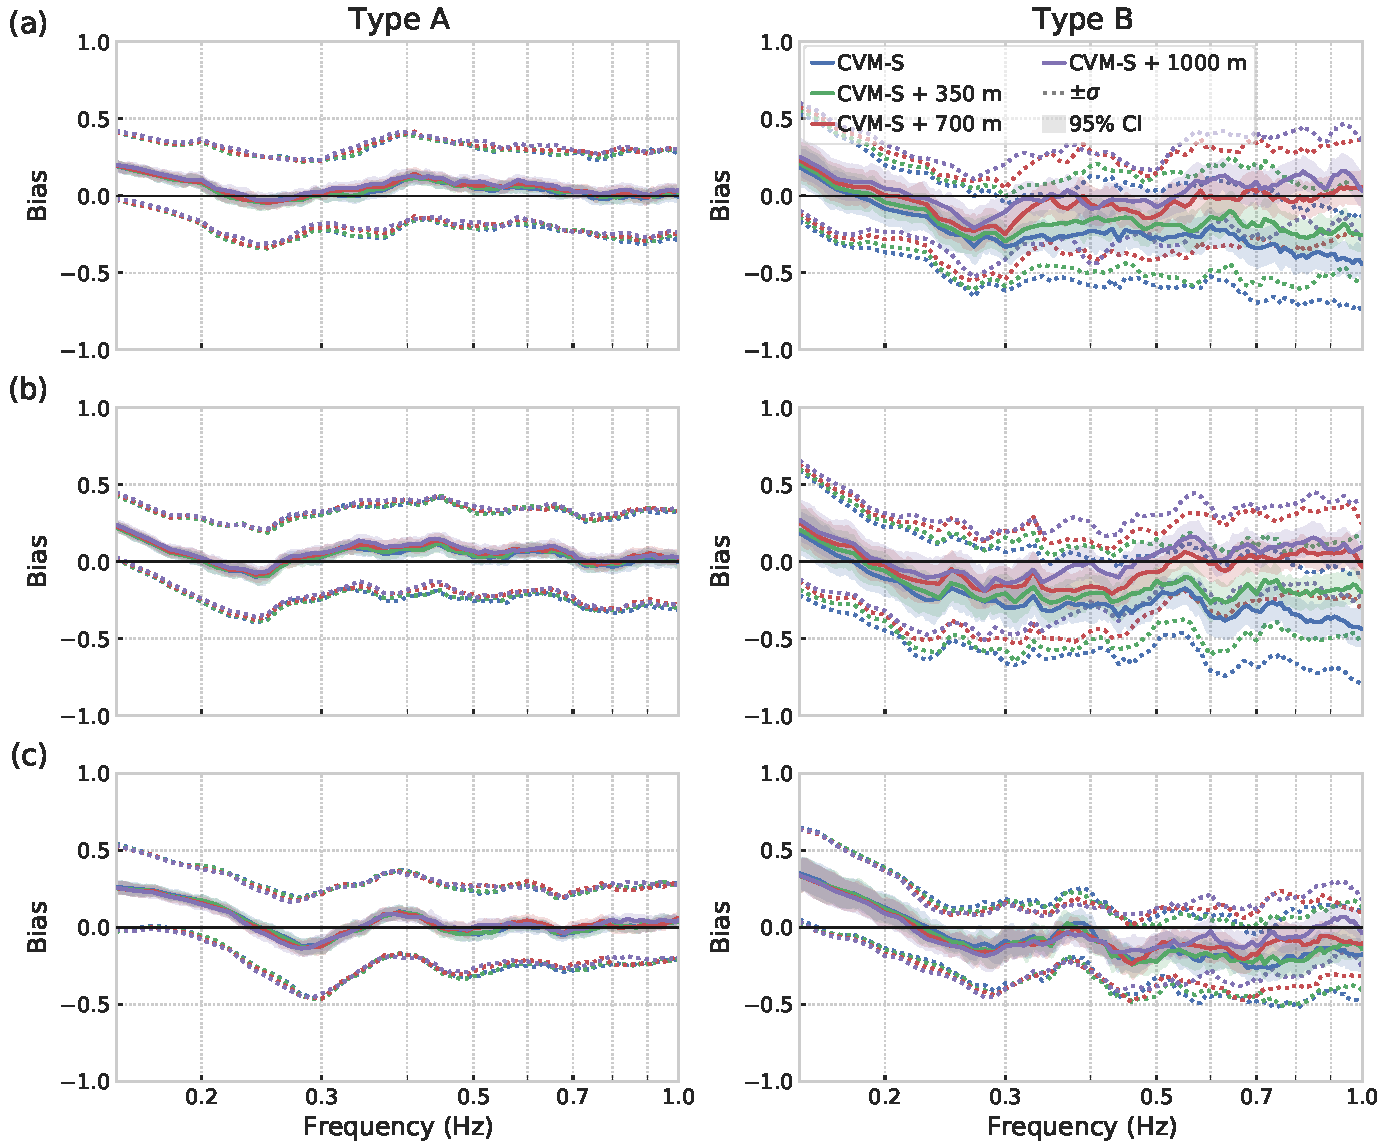
\includegraphics[width=0.9\textwidth]{figures/figure_vs30_9.pdf}
  \caption{Bias of FAS on the (a) east-west, (b) north-south and (c) vertical components, calculated from 3D simulations in CVM-S and with $V_S$ refinements of 350 m, 700 m, and 1000 m. A positive (negative) value depicts overprediction (underprediction). The left (right) column shows soil (rock) sites. The solid line is the median of FAS, where the narrow band is the 95\% confidence interval of the median, and the dashed lines depict the standard deviation centered at the median.}
  \label{fig:vs30-9}
\end{figure}

\clearpage
\begin{figure}[!ht]
  \centering
  \includegraphics[width=0.9\textwidth]{figures/figure_vs30_10.png}
  \caption{Maps of interpolated log10-based FAS bias between four 3D models and data: (a) CVM-S, and CVM-S with refinements of (b) 350 m, (c) 700 m and (d) 1000 m, calculated from the synthetics and records at 259 stations. The warm (cool) colors represent overprediction (underprediction). The circles (triangles) depict soil (rock) sites. Note the log10-based colorbar.}
  \label{fig:vs30-10}
\end{figure}

\clearpage
\begin{figure}[!ht]
  \centering
  \includegraphics[width=0.9\textwidth]{figures/figure_vs30_11.png}
  \caption{Maps of interpolated log10-based FAS bias for two 3D CVMs and data. (a) CVM-S with refinement depth of 350 m and $Q_S=0.15V_S$, and (b) CVM-S with refinement of 1000 m and $Q_S=0.05V_S$. Warm (cool) colors represent overprediction (underprediction). Circles depict soil sites and triangles show rock sites.}
  \label{fig:vs30-11}
\end{figure}

\clearpage
\begin{figure}[!ht]
  \centering
  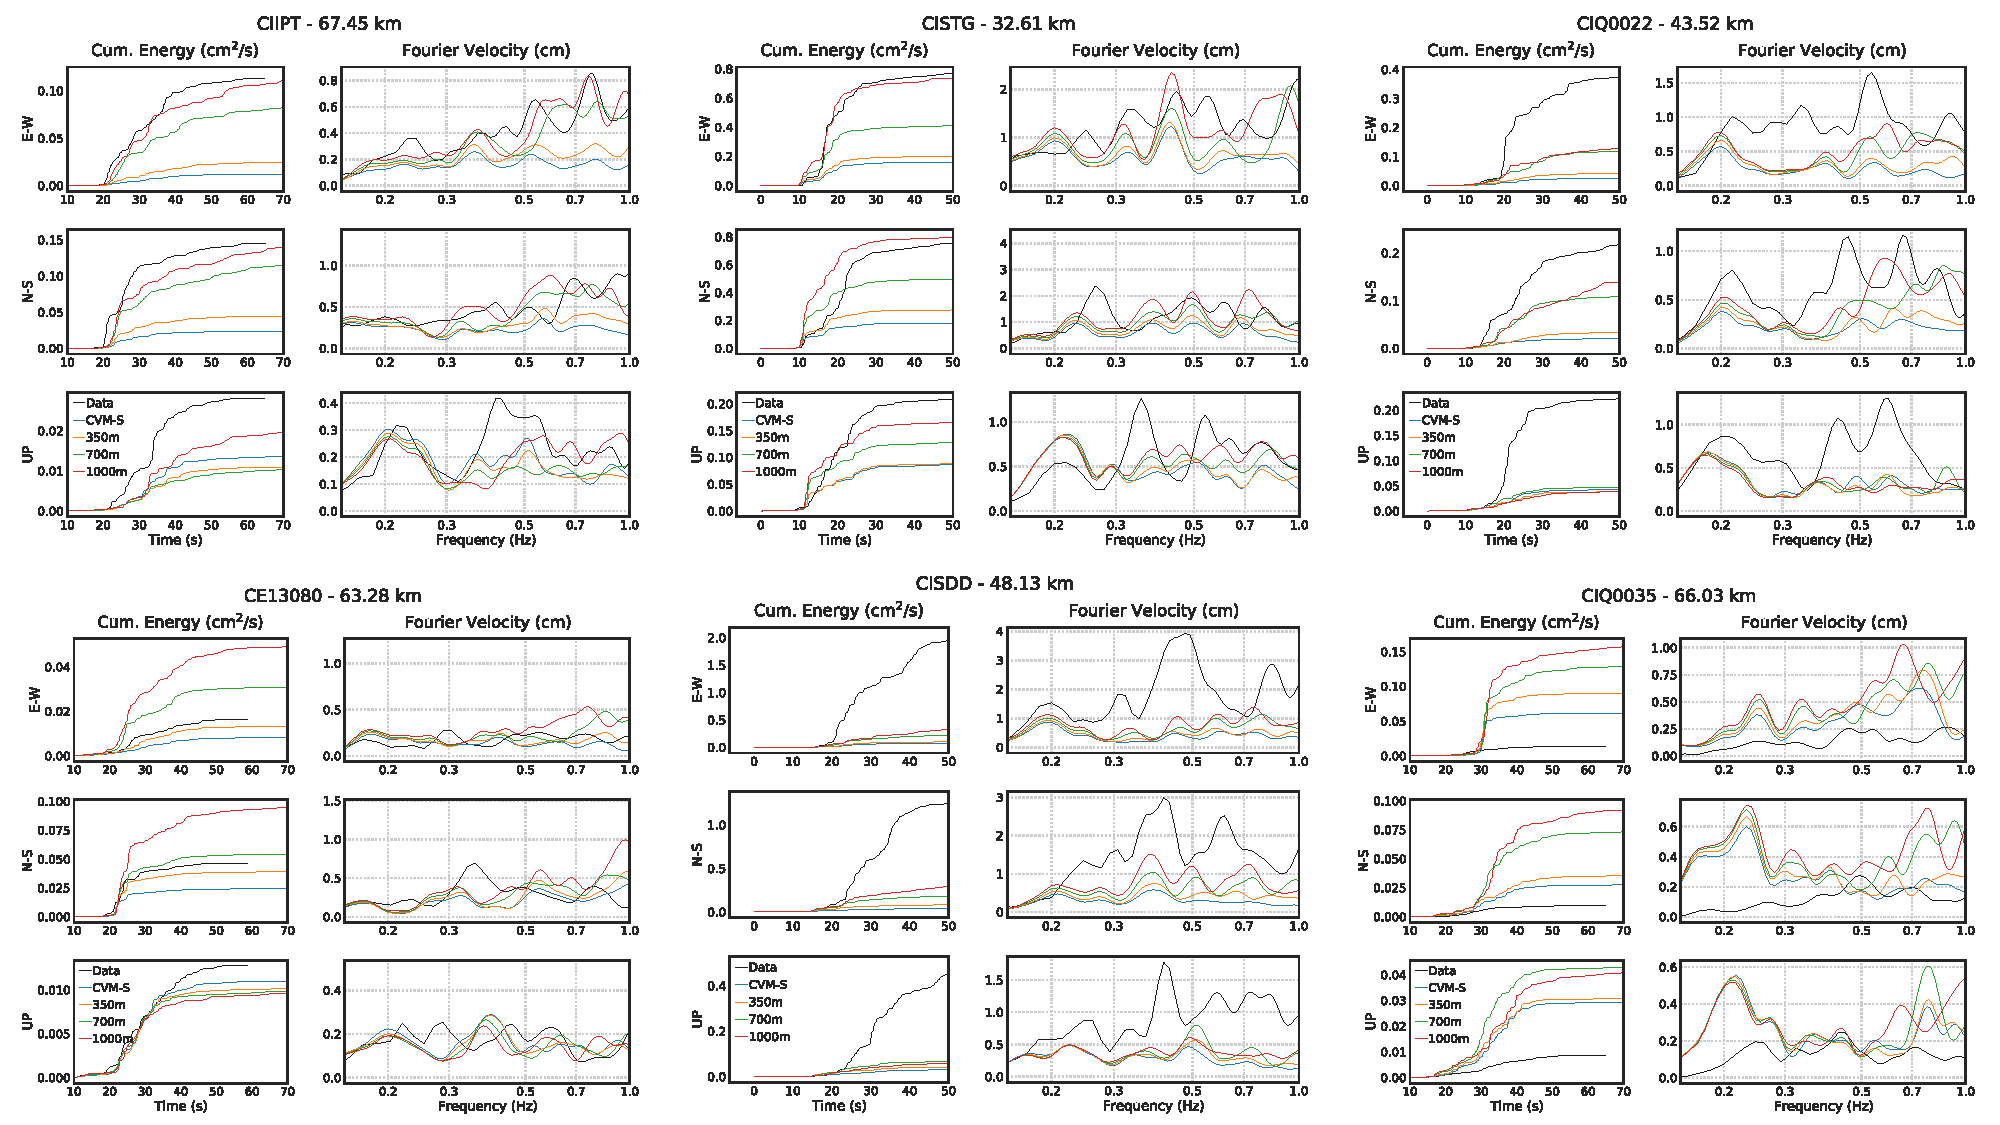
\includegraphics[width=0.9\textwidth]{figures/figure_vs30_12.pdf}
  \caption{Cumulative kinetic energy and Fourier velocity spectra at six rock sites. The subtitles show the names of the sites and their hypocentral distance.
  }
  \label{fig:vs30-12}
\end{figure}

\clearpage
\begin{figure}[!ht]
  \centering
  \includegraphics[width=0.9\textwidth]{figures/figure_vs30_13.pdf}
  \caption{Rock site $V_S$ profiles (defined as surface $V_S$>=1000 m/s) from CVM-S, and CVM-S and CVM-H with (default) \citet{elyVs30derivedNearsurfaceSeismic2010} GTL refinement depth of 350 m.}
  \label{fig:vs30-13}
\end{figure}

\clearpage
\floatsetup[figure]{style=plain,subcapbesideposition=top}
\begin{figure}[!ht]
  \sidesubfloat[]{\includegraphics[width=0.4\textwidth]{figures/figure_vs30_14a.png}\label{fig:vs30-14a}} \hfil
  \sidesubfloat[]{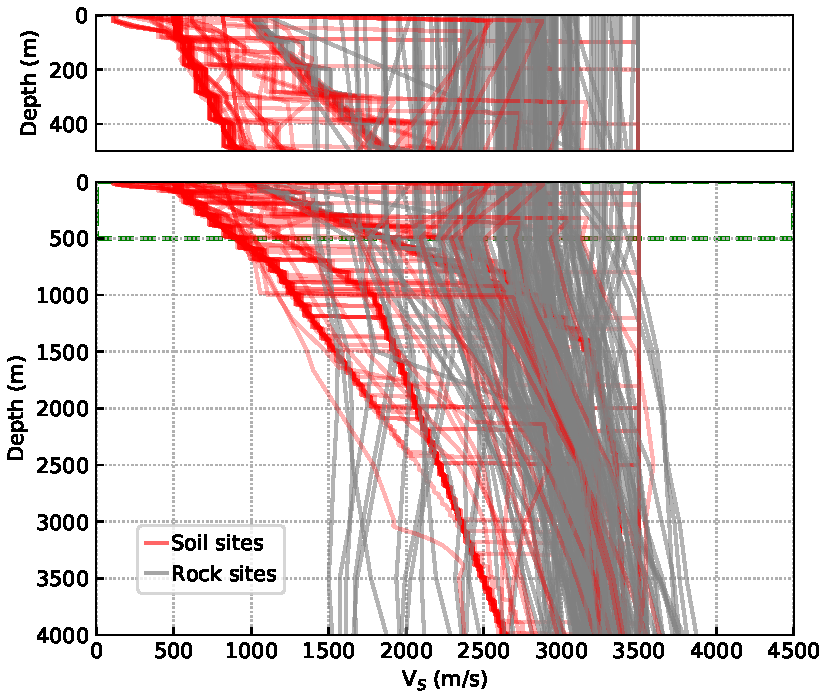
\includegraphics[width=0.45\textwidth]{figures/figure_vs30_14b.pdf}\label{fig:vs30-14b}} % \\[\baselineskip]%
  \caption{ (a) $V_S$ profile sample locations in California. Triangles denote rock sites and circles denote soil sites, and (b) extracted $V_S$ profiles. The top panel zooms into the top 500 m. }
  \label{fig:vs30-14}
\end{figure}

\clearpage
\begin{figure}[!ht]
  \centering
  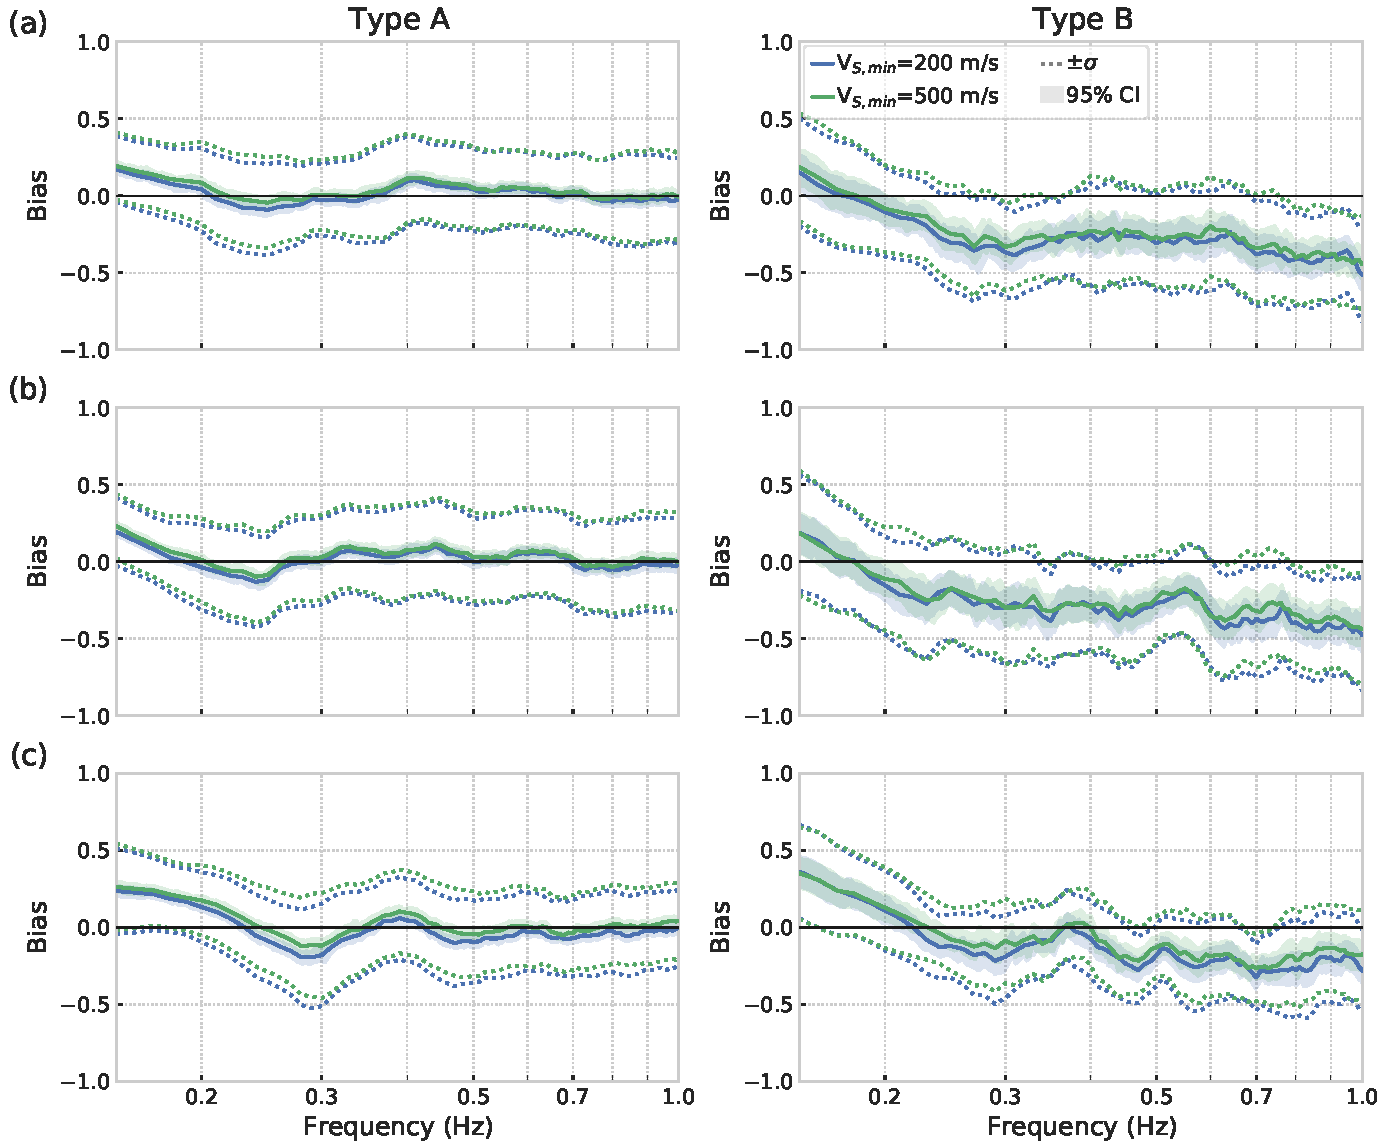
\includegraphics[width=0.9\textwidth]{figures/figure_vs30_S1.pdf}
  \caption{Bias of FAS of the (a) east-west, (b) north-south and (c) vertical component, calculated from 3D simulations in CVM-S with $V_S$ refinement depths of 350 m and 1000 m along with attenuation models $Q_S=0.05V_S$, $Q_S=0.1V_S$, and $Q_S=0.15V_S$. A positive (negative) value means overprediction (underprediction). The left (right) columns show soil (rock) sites. The solid line is the median of FAS, where the narrow band is the 95\% confidence interval of the median, and the dashed lines depict the standard deviation centered at the median.}
  \label{fig:vs30-S1}
\end{figure}

\clearpage
\begin{figure}[!ht]
  \centering
  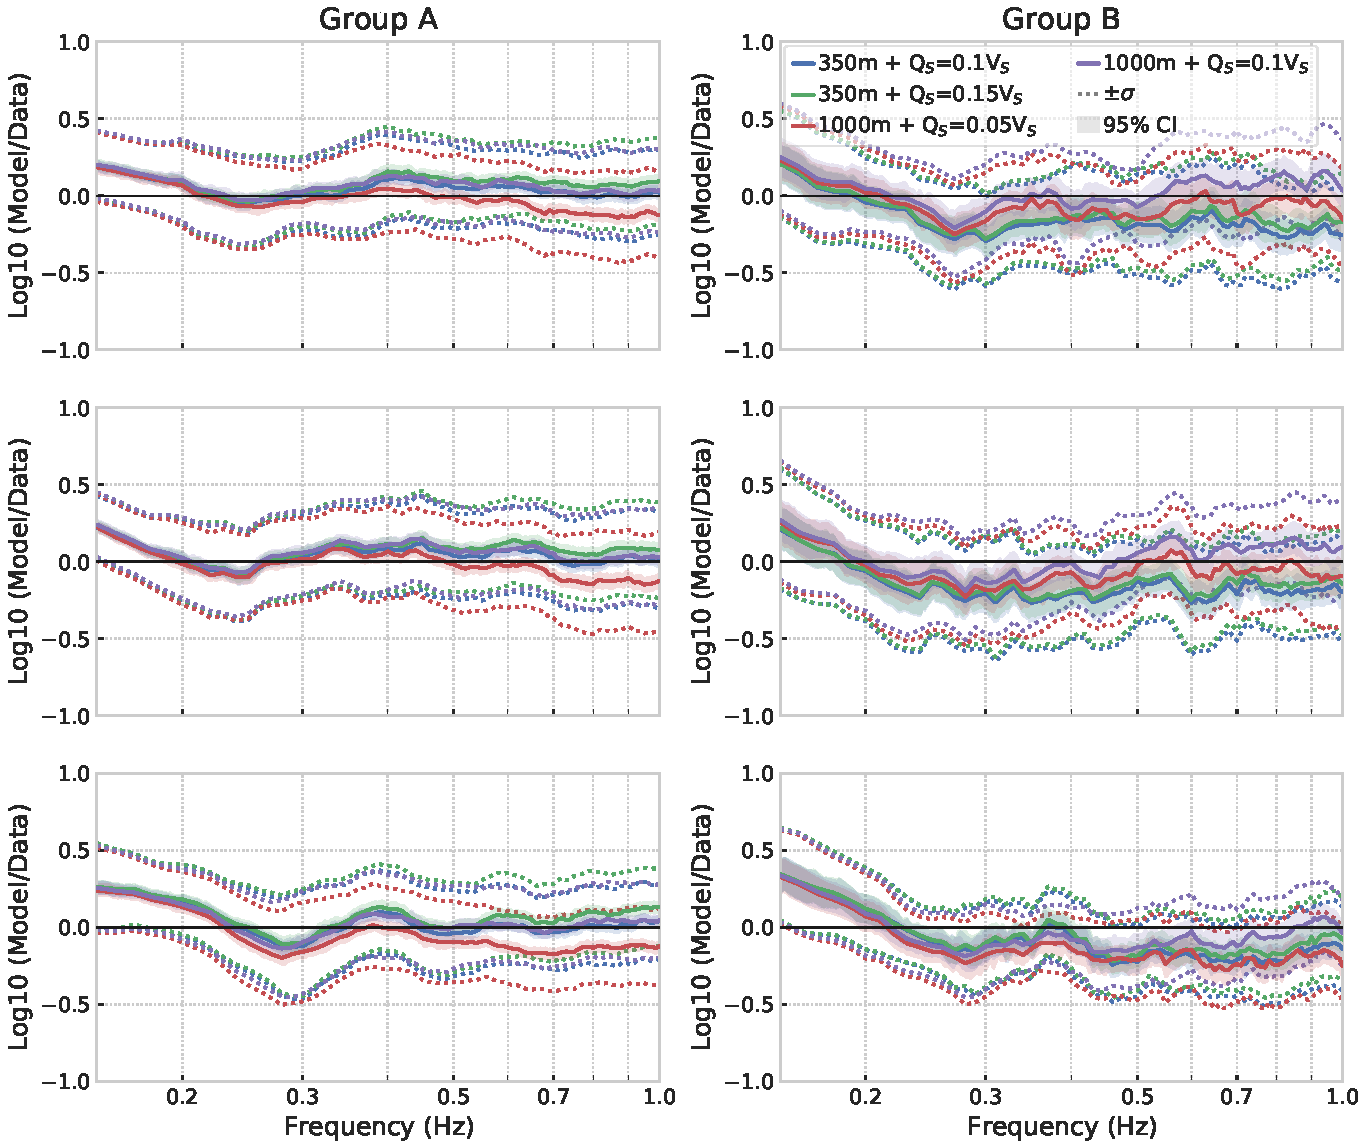
\includegraphics[width=0.9\textwidth]{figures/figure_vs30_S2.pdf}
  \caption{Average FAS bias for frequencies between 0.15-1 Hz at rock sites plotted as a function of site surface $V_S$ for (a) three-component average, (b) east-west, (c) east-west and (d) vertical components. The shades represent 95\% confidence intervals estimated using bootstrap.}
  \label{fig:vs30-S2}
\end{figure}

%% supplement
\setcounter{table}{0}
\setcounter{figure}{0}
\numberwithin{figure}{chapter}
\numberwithin{table}{chapter}
\renewcommand{\thetable}{S\arabic{chapter}.\arabic{table}}
\renewcommand{\thefigure}{S\arabic{chapter}.\arabic{figure}}
\newpage
\section*{Supplementary Materials}
\addcontentsline{toc}{section}{\protect\numberline{}Supplementary Materials}

This supplement includes.




\renewcommand{\thetable}{\arabic{table}}
\renewcommand{\thefigure}{\arabic{figure}}

\numberwithin{figure}{chapter}
\numberwithin{table}{chapter}

%\endrefsection